\documentclass[a4paper]{article}
\usepackage[utf8]{inputenc}
\usepackage[spanish, es-tabla, es-noshorthands]{babel}
\usepackage[table,xcdraw]{xcolor}
\usepackage[a4paper, footnotesep = 1cm, width=20cm, top=2.5cm, height=25cm, textwidth=18cm, textheight=25cm]{geometry}
%\geometry{showframe}

\usepackage{tikz}
\usepackage{amsmath}
\usepackage{amsfonts}
\usepackage{amssymb}
\usepackage{float}
\usepackage{graphicx}
\usepackage{caption}
\usepackage{subcaption}
\usepackage{multicol}
\usepackage{multirow}
\setlength{\doublerulesep}{\arrayrulewidth}
\usepackage{booktabs}

\usepackage{hyperref}
\hypersetup{
    colorlinks=true,
    linkcolor=blue,
    filecolor=magenta,      
    urlcolor=blue,
    citecolor=blue,    
}

\newcommand{\quotes}[1]{``#1''}
\usepackage{array}
\newcolumntype{C}[1]{>{\centering\let\newline\\\arraybackslash\hspace{0pt}}m{#1}}
\usepackage[american]{circuitikz}
\usetikzlibrary{calc}
\usepackage{fancyhdr}
\usepackage{units} 

\graphicspath{{../Calculos-Potencia/}{../Caracteristicas/}{../Consideraciones/}{../Gain-Stage/}{../Input-Stage/}{../Output-Stage/}{../Simulaciones/}{../Alimentacion/}{../Conclusiones/}}

\pagestyle{fancy}
\fancyhf{}
\lhead{22.12 Electrónica II}
\rhead{Mechoulam, Lambertucci, Rodriguez, Londero, Scala}
\rfoot{Página \thepage}

\begin{document}

\subsection{Introducción}
Se realizaron simulaciones en LTSpice del circuito propuesto, así también se comprobó que los resultados teóricos concuerdan con las simulaciones, ademas se tuvo especial cuidado a la hora de evaluar que transistores y resistores usar en las etapas tal que no haya problemas de potencia, aqui se muestran las tensiones y potenicas relevantes del circuito en cuanto a la elección crítica de componentes.\\
Comenzando por los emisores comunes la potencia se encuentra cerca del máximo y la tensión Vce en un rango seguro.
\begin{figure}[H]
	\centering
	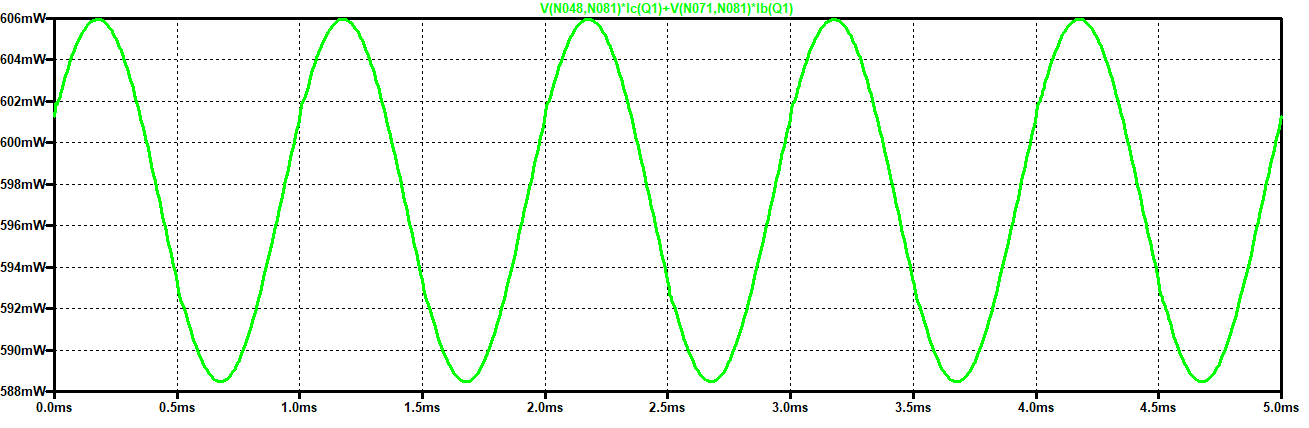
\includegraphics[width=\textwidth]{ImagenesSimulaciones/PEC1.png}
	\caption{Potencia sobre un emisor común sin carga activa.}
	\label{fig:pec1}
\end{figure}
\end{document}